%!TEX root = ../../../thesis.tex

\section{The streaming potential cell}
\label{sect:streamingPotentialCell}

The streaming potential cell is a device that uses water flow to separate charge.
It is particularly promising as a harvester due to its lack of moving parts.
This chapter starts by explaining how a streaming cell makes use of the interfacial double layer to separate charge.
Then I construct a crude cell and measure its performance.
This is followed by a mathematical investigation of the streaming cell.

For the sake of brevity, the term `cell' in this chapter shall refer to a streaming potential cell.
And the term `interface' refers to the interface, or boundary, between solid and liquid matter.
Unless otherwise stated, it should be assumed that I am describing the liquid side of the interface.
The solid body typically plays no role, apart from the surface charge it holds.

\begin{figure}
    \centering
    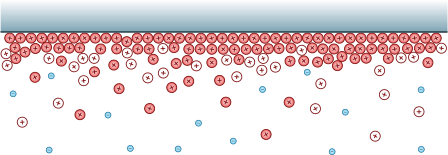
\includegraphics{content/pt1/01-PowerHarvesting/graphics/doubleLayerOnWall}
    \caption{\label{fig:doubleLayerOnWall}Formation of a double layer on a wall}
\end{figure}

Figure \ref{fig:doubleLayerOnWall} shows the formation of a double layer at the interface of a charged wall.
A higher density of positively charged ions, or cations, sit close to the interface.
The density of these cations reduces as the distance to the interface increases.
Also, the density of negatively charged ions, or anions, increases with the distance from the interface.

Now imagine a very small cavity filled with an electrolyte.
A simplified representation of such a cavity is shown in figure \ref{fig:ionsInABox}.
If the walls of the cavity hold no surface charge then the ions distribute evenly throughout the volume.
That is to say, the ions in the liquid are not electrically influenced by the walls.
With the application of surface charge - the counter-ions migrate to the walls.
As the density of counter-ions has increased at the interface, a void of cations remains within the cavity.
This is a very simplistic introduction to the method of double layer charge separation.

\begin{figure}
    \centering
    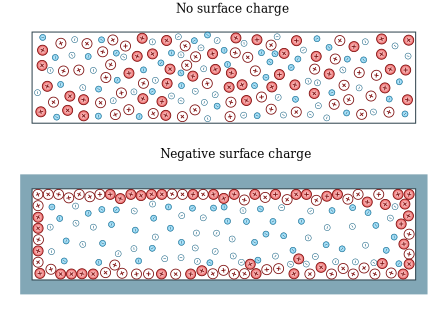
\includegraphics{content/pt1/01-PowerHarvesting/graphics/ionsInABox}
    \caption{\label{fig:ionsInABox}Charge distribution in a charged cavity versus a non-charged cavity}
\end{figure}

Charge separation, as described in the previous example, is not enough to develop electrical power.
Two reasons electrical power can't be extracted directly from a double layer are:
\begin{itemize}
    \item The counter-ions of a double layer are electrostatically bound to the interface.
        Removing these ions from the interface requires work.
    \item A double layer shields the electric field created by surface charge at the interface.
        Once the layer has created an equal and opposite field at the interface, the remaining liquid within the volume is unaffected by charge at the interface.
\end{itemize}

A streaming potential cell needs to convert power behind flowing liquid into electrical power.



A cell separates charge using water pressure

Figure \ref{fig:doubleLayerOnWall} shows how ions in a double layer concentrate at the boundary between solid and liquid. 
This boundary will be referred to as `the interface'.


about how this happens is discussed in the introduction.
The cell does this by using a double layer to draw charge into a carefully constructed cavity.
The walls of the cavity hold a surface charge to create the double layer.

a cavity in orde with 
by within
a cavity forcing water through narrow cavities. This phenomenon is understood
and is used in colloidal science to determine what's called the zeta potential
of an interface \cite{Gu2000,Scales1992,Daiguji2004,VanderHeyden2006,Mala1997}.
Although this phenomenon isn't new, using it to generate useful amounts of
electrical energy is. This chapter will investigate the application of
streaming potentials to energy harvesting for the purposes of running a smart
water meter.

% At the boundary between a liquid and a solid, be it a molecule or the wall of
% a container, there is a possibility for an electrical potential. This
% electrical potential exists at the interface between the liquid and the solid
% and is the underlying mechanism by which the streaming potential cell
% operates. To understand how this electrical potential is able to separate
% charge as it does in a streaming potential cell we will first observe what
% happens when a solid suspended in liquid, as is shown in Figure
% \ref{Figure_Diagram_ZetaPotential_and_SlippingPlane}.


\begin{figure} \centering
    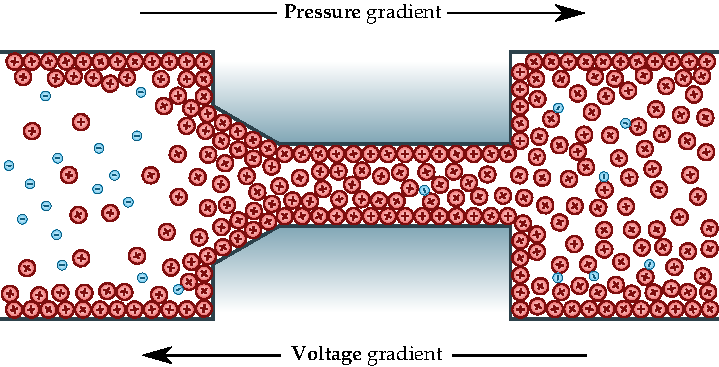
\includegraphics{content/pt1/01-PowerHarvesting/graphics/streamingCellPrinciple}
    \caption{\label{fig:streamingCellPrinciple}The general principle of
        operation of the streaming potential cell} \end{figure} In this
diagram, a the negatively charged solid is surrounded by layers of positively
charged ions that are electrostaticly attracted to the surface of the solid.
Near the surface of the solid, tightly bound, positively charged ions are
packed together and are largely immobile.  These ions reside in what is called
the Stern Layer. After this layer is a shell of less densely packed and
somewhat mobile ions that are still bound to the solid. At the edge of this
shell is what is called the slipping plane, which is the point at which ions
are no-longer bound to the solid. The electrical potential at this slipping
plane is termed the $\zeta$ potential (zeta potential). ``This zeta potential
is directly related to the interaction between the solid particles themselves
when they are suspended in a liquid and thus determines the stability of the
suspension solutions'' \cite{Gu2000}.

% \begin{figure} \begin{centering}
% 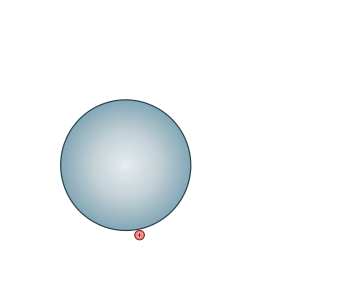
\includegraphics[scale=0.12]{content/pt1/01-PowerHarvesting/Diagram_of_zeta_potential_and_slipping_plane_thesisEdit}
% \par\end{centering}

% \centering{}\protect\caption{\label{Figure_Diagram_ZetaPotential_and_SlippingPlane}Diagram
% showing the ionic concentration and potential difference as a function of
% distance from the charged surface of a particle suspended in a dispersion
% medium.} \end{figure}


Now lets look at the case where the geometry is such that the surface charge
resides on the walls of a channel through which the liquid can flow, as is
shown in Figure \ref{Figure_Diagram_ZetaPotential_and_in_a_channel}.  By
setting the width of the channel such that the double layer formed on each of
the sides partially overlap, the channel will be predominantly occupied by ions
of the opposite polarity to that of the surface charge at the solid to liquid
interface. This configuration has the effect of promoting the transport of
those ions across the channel with the application of a pressure differential
across the channels length.

%\begin{figure}
%\centering{}\includegraphics[scale=0.12]{content/pt1/01-PowerHarvesting/Diagram_of_zeta_potential_in_a_channel_thesisEdit}\protect\caption{\label{Figure_Diagram_ZetaPotential_and_in_a_channel}Diagram
%showing the ionic concentration and potential difference as a function of
%distance from the charged surfaces of a micro-channel.} \end{figure}



\section{Replicating an experiment}

There are many papers describing experiments with streaming potential cells
\cite{Gu2000,Mala1997,Scales1992,VanderHeyden2006} of which we have chosen one
by Yongan Gu and Dongqing Li \cite{Gu2000} to attempt to replicate. This paper
was chosen for its detailed description of the experimental procedure used,
including the brands and model numbers of the equipment used. Our experimental
procedure is based upon this paper however we have modified certain areas of
the experiment to accommodate for the resources available to us. For a list of
the materials used to construct the channels, see Table
\ref{Table_StreamingCell_MaterialsUsed}.


\subsection{\label{sub:Experimental-Procedure}Experimental Procedure}


\subsubsection{Construction}

\begin{figure}[p] \begin{centering}
        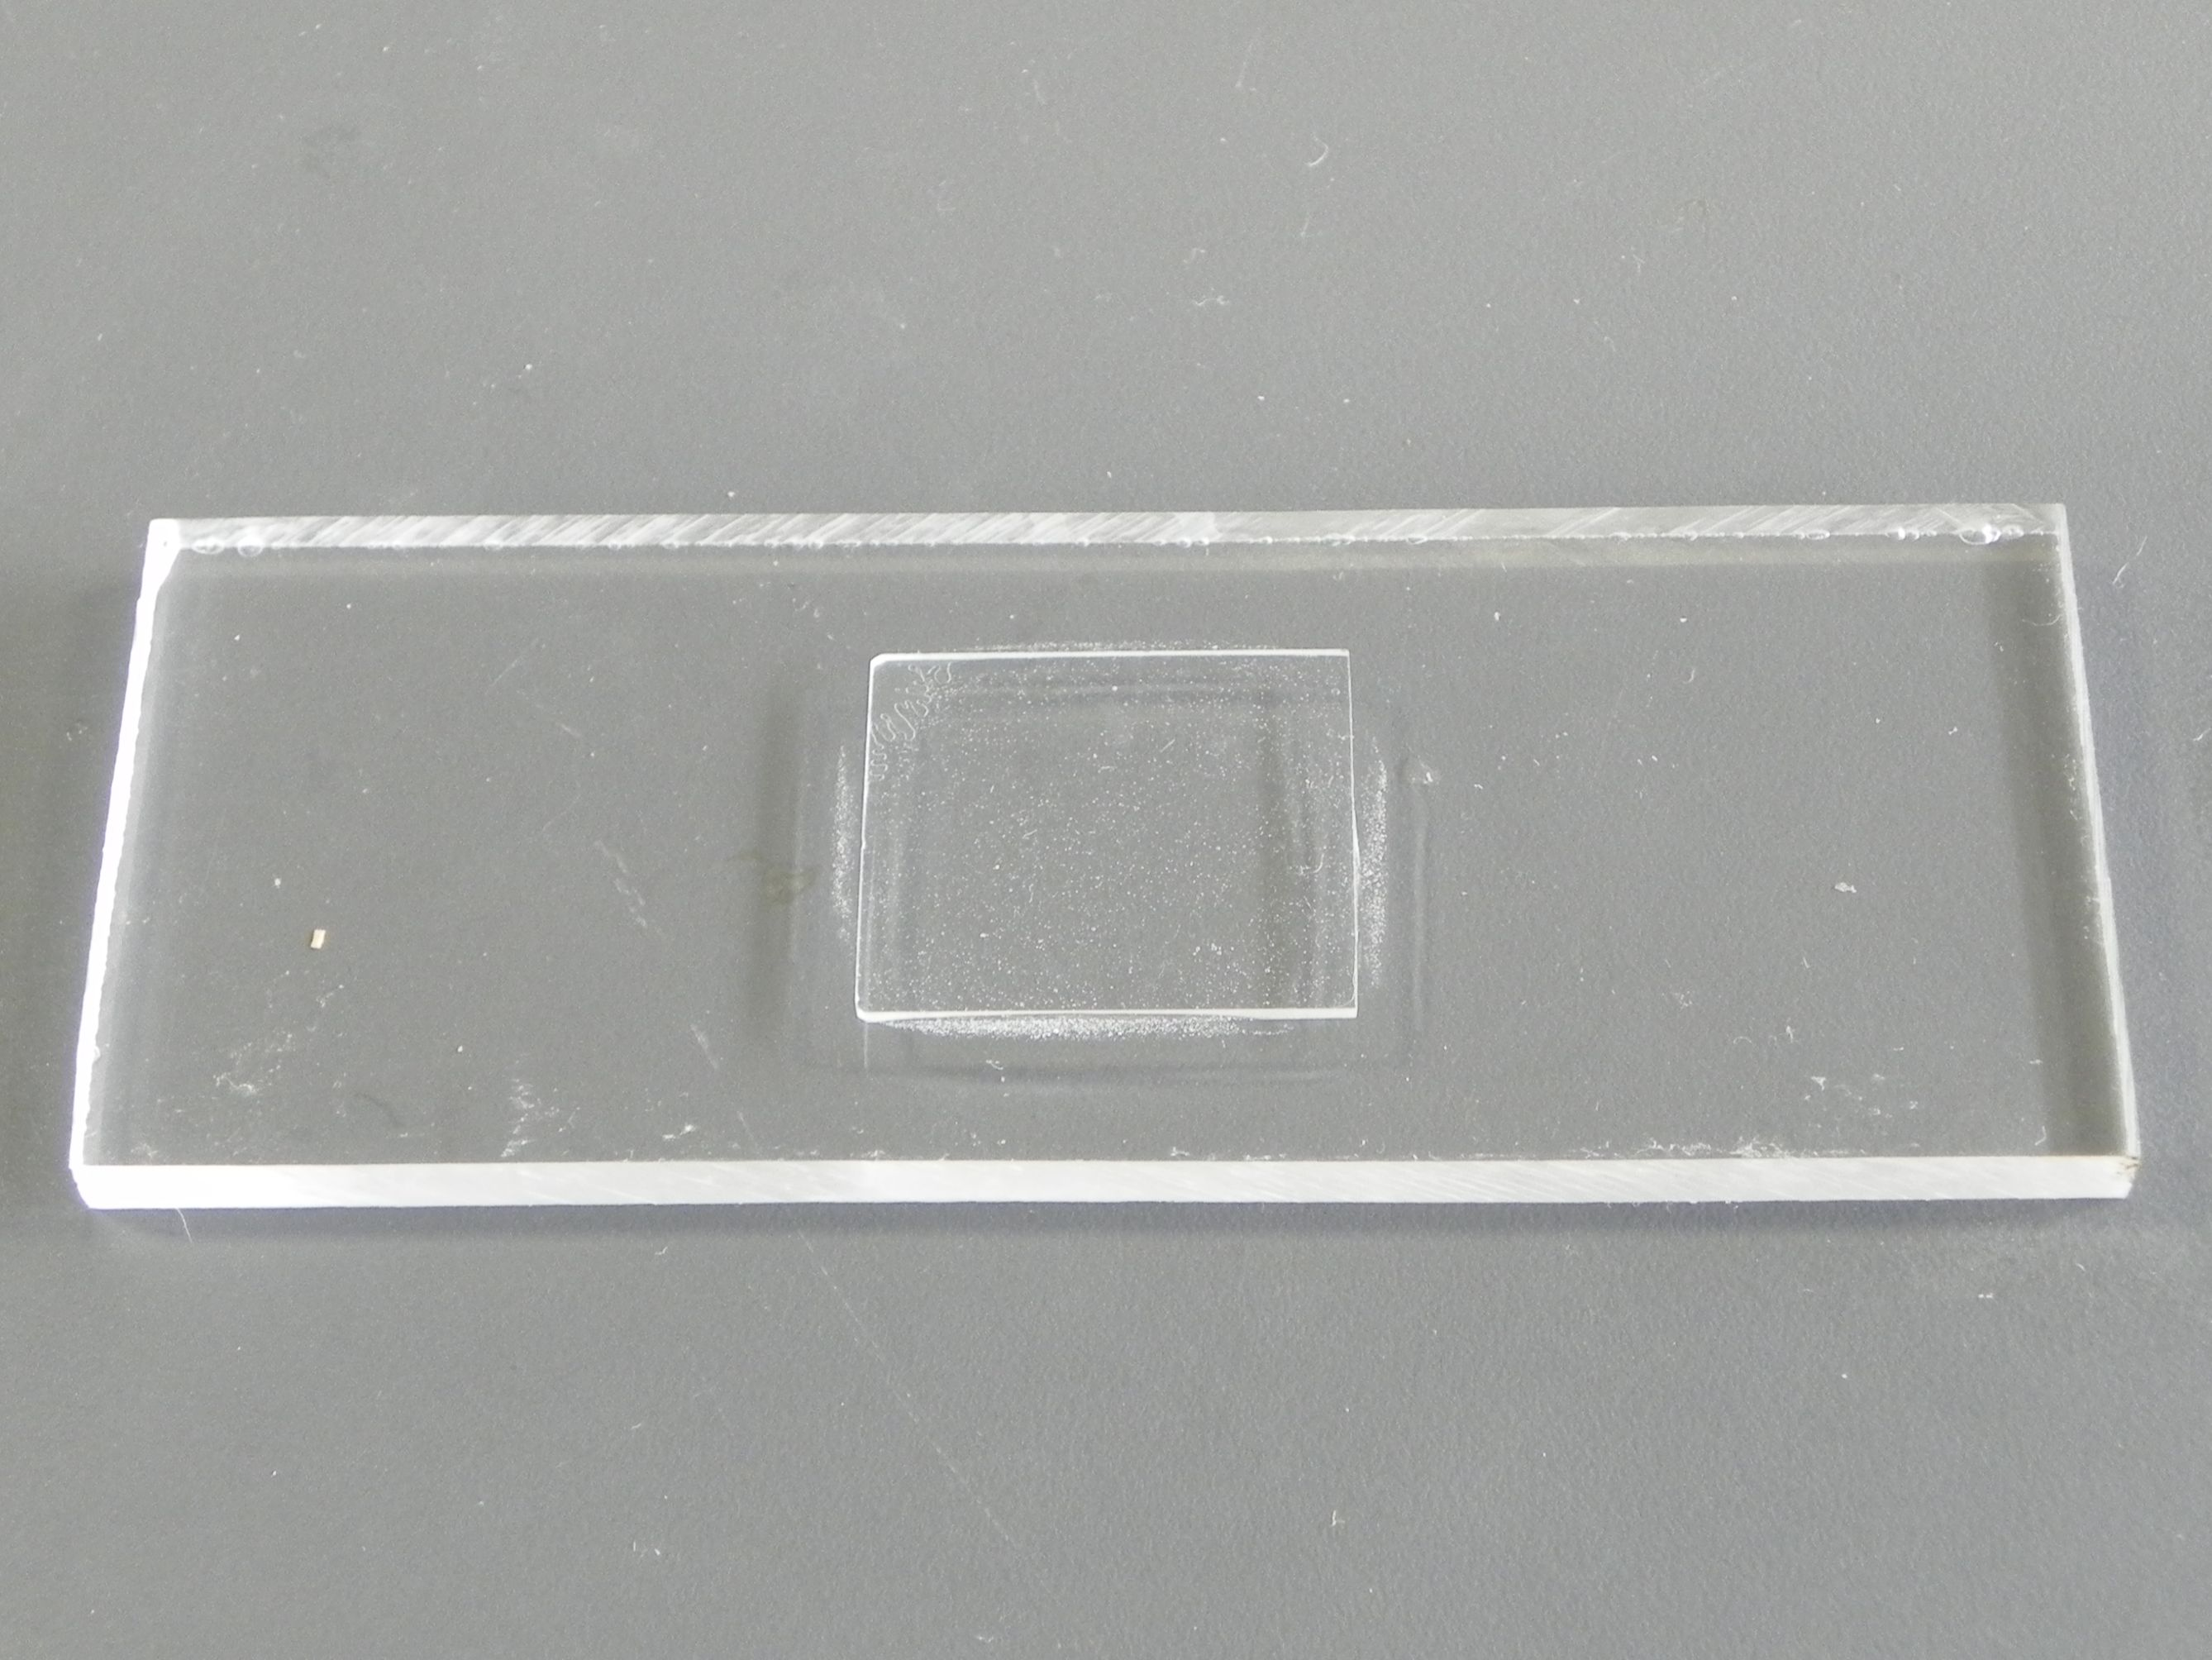
\includegraphics[width=0.5\textwidth]{content/pt1/01-PowerHarvesting/graphics/Photo_streamingPotential_Assembly_Step1.JPG}
        \par\end{centering}

\centering{}\protect\caption{\label{Photo_streamingPotential_Assembly_Step1}Photo
    showing half of a glass slide glued to acrylic base plate} \end{figure}
\begin{figure}[p] \begin{centering}
        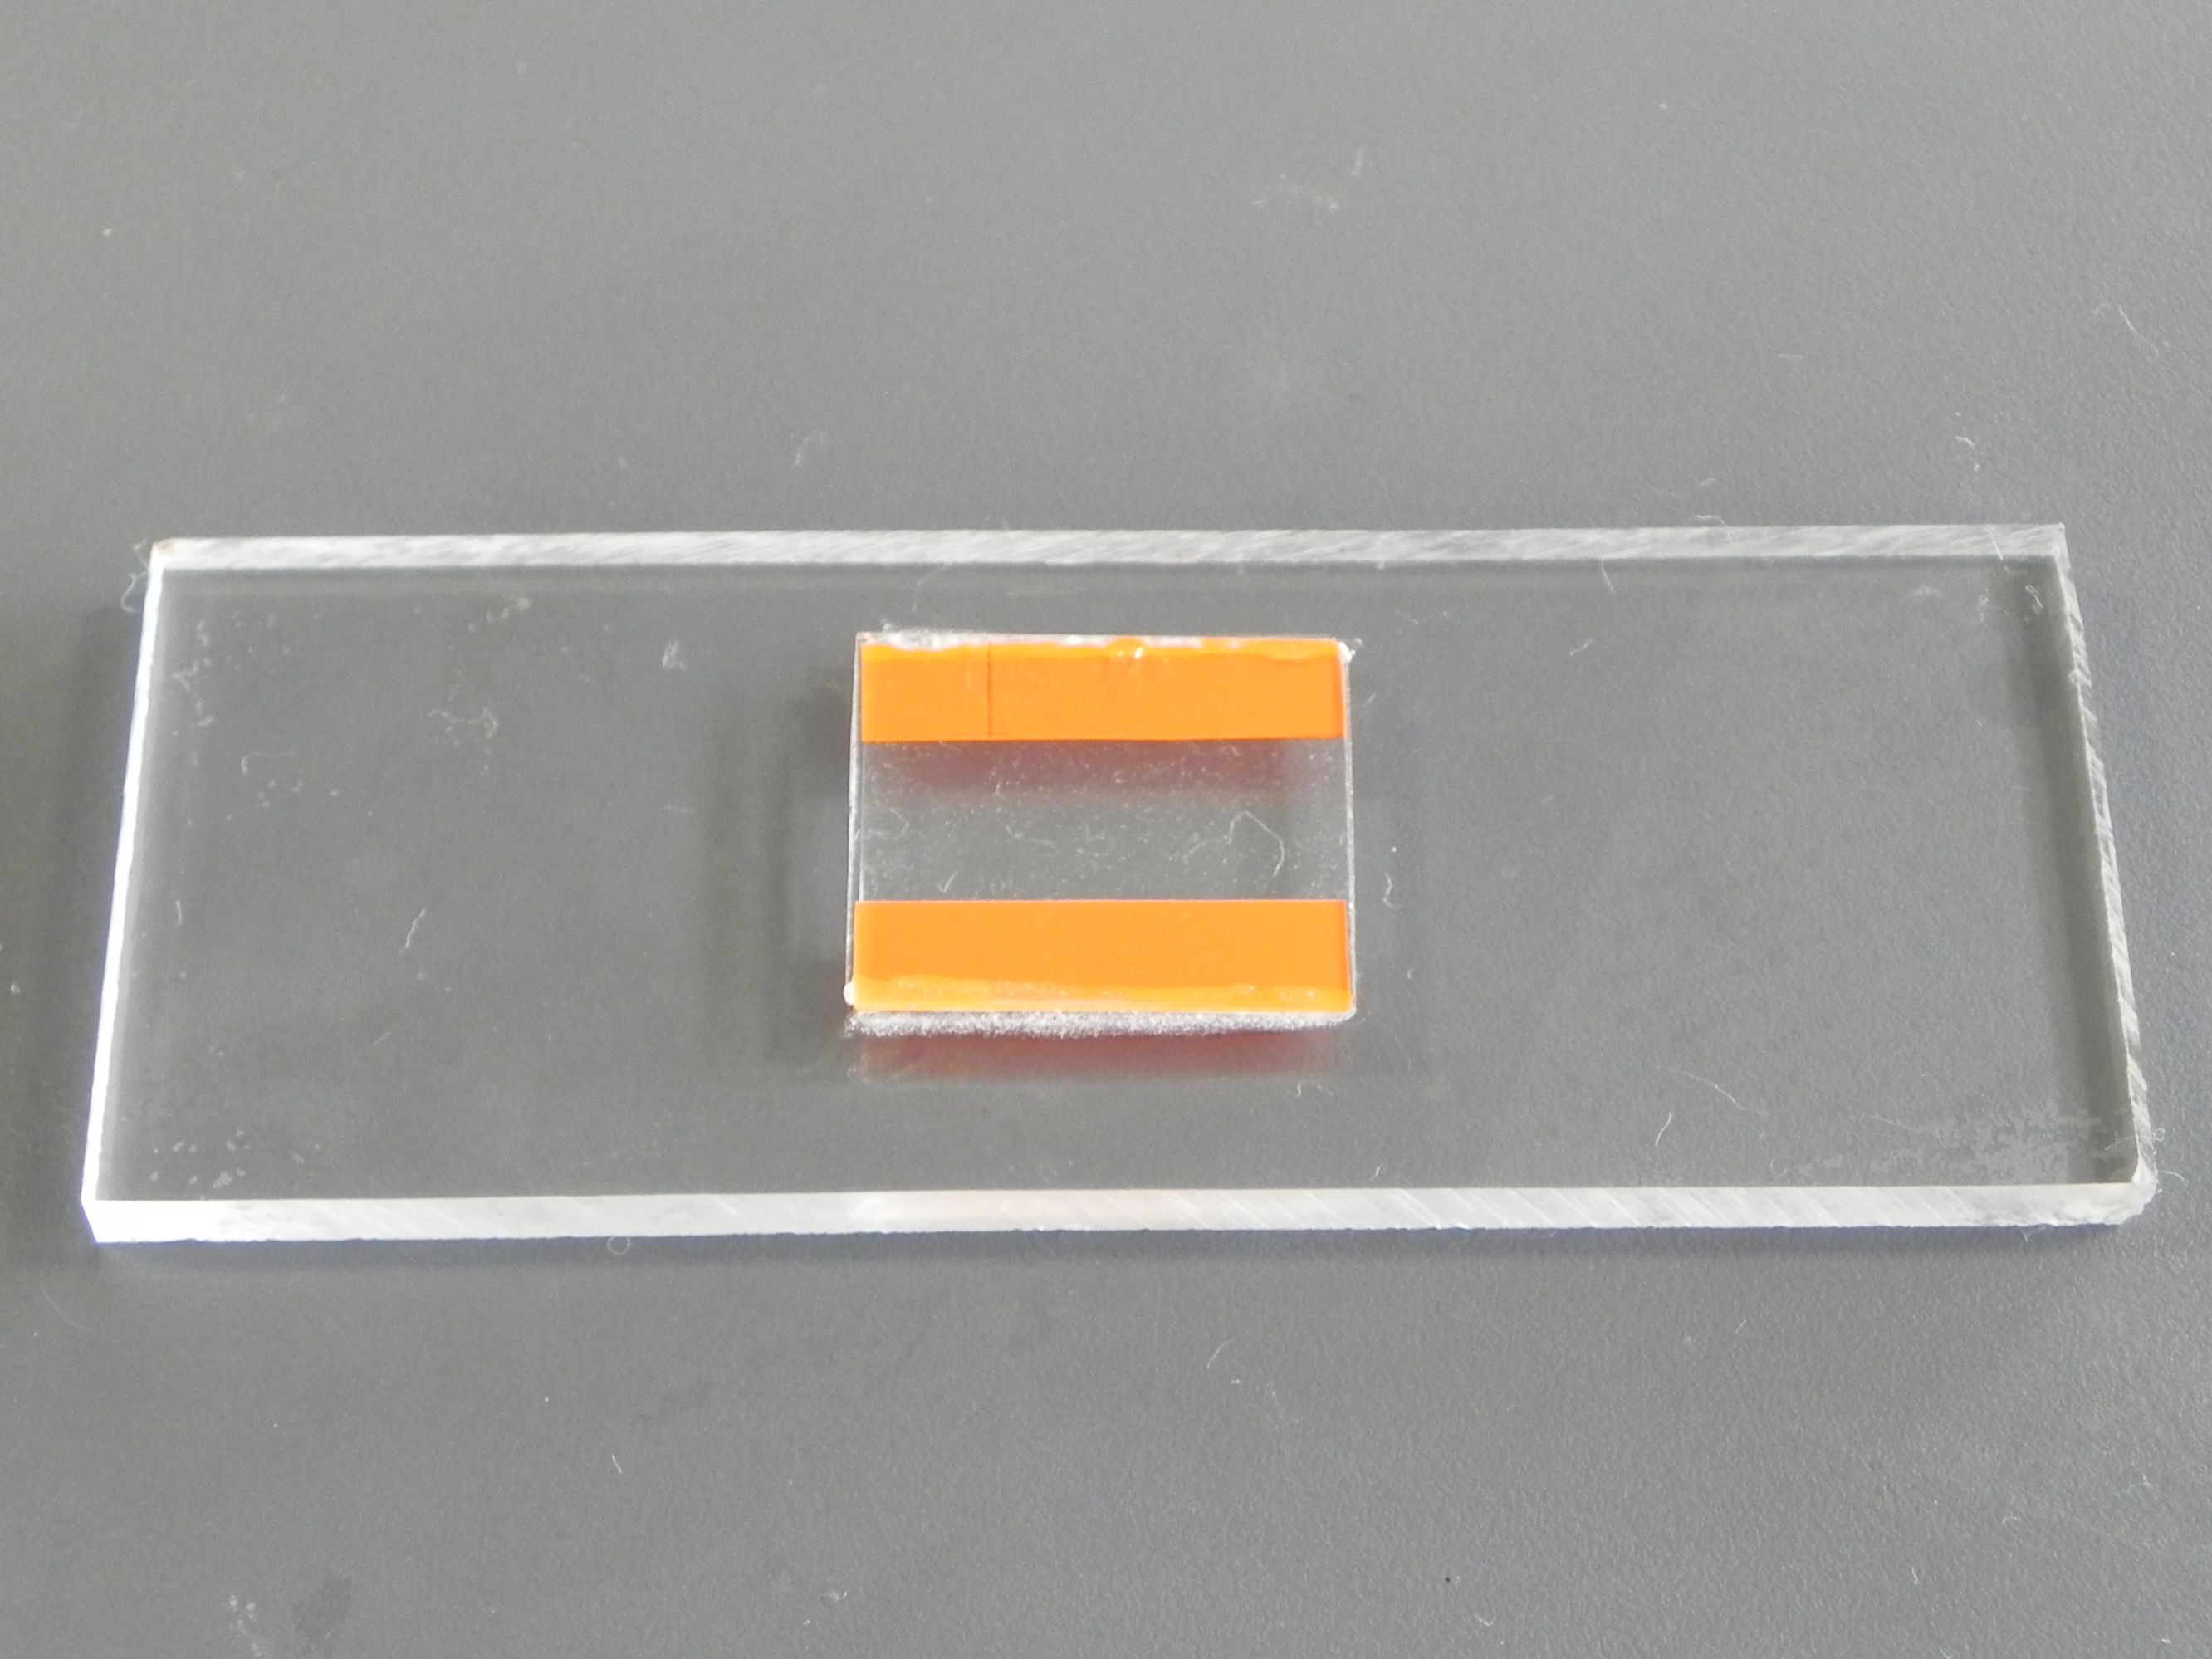
\includegraphics[width=0.5\textwidth]{content/pt1/01-PowerHarvesting/graphics/Photo_streamingPotential_Assembly_Step2.JPG}
        \par\end{centering}

\centering{}\protect\caption{\label{Photo_streamingPotential_Assembly_Step2}Photo
    showing shims sandwiched between two slide halves} \end{figure}
\begin{figure}[p] \begin{centering}
        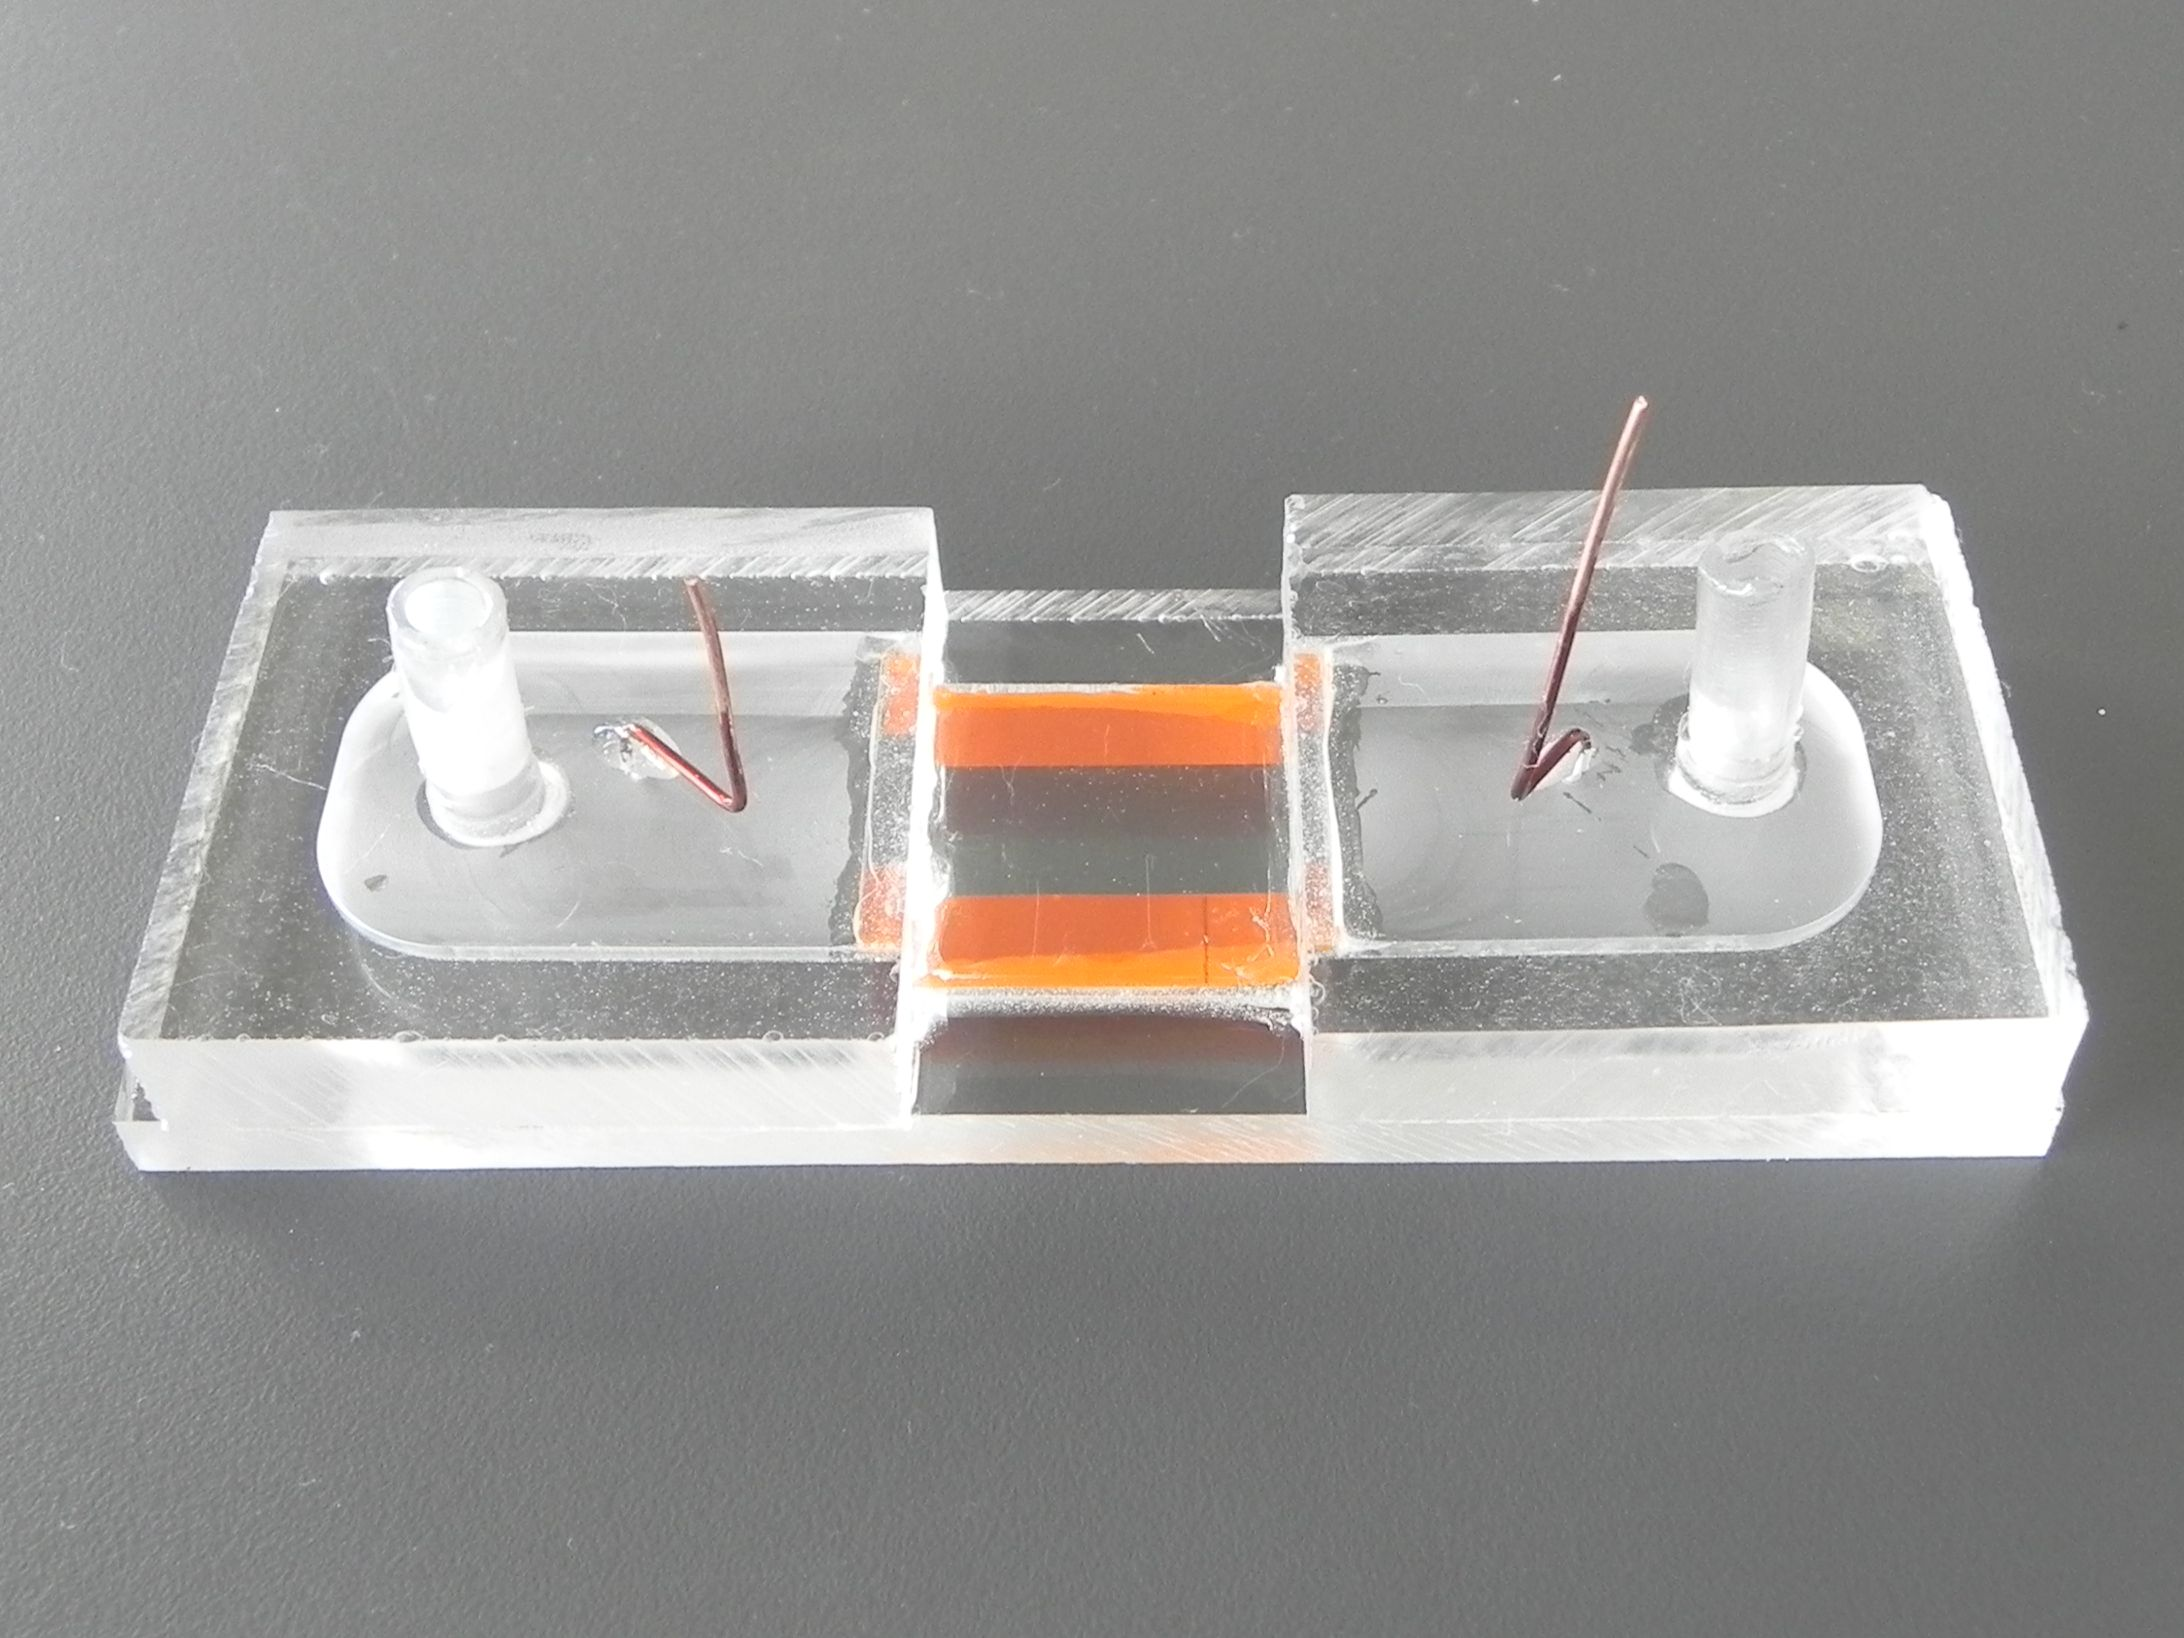
\includegraphics[width=0.5\textwidth]{content/pt1/01-PowerHarvesting/graphics/Photo_streamingPotential_Assembly_Step3.JPG}
        \par\end{centering}

\centering{}\protect\caption{\label{Photo_streamingPotential_Assembly_Step3}Photo
    showing final assembly} \end{figure} \begin{figure}
\begin{tabular}{|c|c|c|} \hline Microscope slides & Sail Brand & JIA 7101WT -
    26 x 76mm\tabularnewline \hline Shims & Garlock & Colorplast - 50$\,\mu$m,
    80$\,\mu$m, 120$\,\mu$m and 250$\,\mu$m\tabularnewline \hline Epoxy &
    Selleys & Araldite - Ultra Clear Resin\tabularnewline \hline Pressure
    Sensor & Honeywell & 24PC15SMT - 0 -- $\pm$15 PSI\tabularnewline \hline
\end{tabular}

\protect\caption{\label{Table_StreamingCell_MaterialsUsed}Table of materials
    used to construct the streaming potential cells} \end{figure}


First, glass microscope slides where cut in half to give panels of glass that
where approximately 26 x 38mm. Once such glass panel can be seen in Figure
\ref{Photo_streamingPotential_Assembly_Step1}.  Next, two pieces of shim
material where placed on either side of the glass panel with a small amount of
epoxy, on top of which another glass panel was placed. Pressure was applied to
the panels pressing them together while the epoxy set to create the channel
that can be seen in Figure \ref{Photo_streamingPotential_Assembly_Step2}. Each
channel was photographed under microscope once set to determine the height of
the channel created. Finally, acrylic couplers where mounted over each end,
again by the use of epoxy. These couplers allowed the water to be forced
through the channel while providing mounting for the voltage sensing wires. The
final assembly is shown in Figure
\ref{Photo_streamingPotential_Assembly_Step3}.


\subsubsection{Measurement}

Each assembly was connected between the tap and drain of a lab basin.  To
facilitate measurement of the pressure gradient across the channel, a pressure
transducer was placed across the input and output ports of the channel
assembly. Single core copper wire was used to measure voltage gradients across
the channel. These wires where epoxied into the couplers to reduce leaks. To
conduct the measurements an Agilent E5270B Precision Measurement Mainframe was
used, which has an input impedance of 10${\displaystyle \, T\Omega}$. The high
input impedance of this machine ensures that the measurements are not disturbed
by current leaking through the measurement device. The E5270 was responsible
for measuring the output of the pressure transducer and the voltage across the
channel.


\subsection{Results}

Ten cavities ranging in height from 26$\,\mu m$ to 245$\,\mu m$ where built and
measured. Individual plots showing pressure applied versus voltage developed
are shown in Appendix \ref{sec:Appendix-Streaming-Potential-Cell}.  For
convenience, a graph with the steepest voltage per pressure gradient is shown
in Figure \ref{fig:streamingCell_voltVsPress_52um_convienient}, which resulted
from using a cell with a height of 52$\,\mu m$.

\begin{figure}[H] \centering
    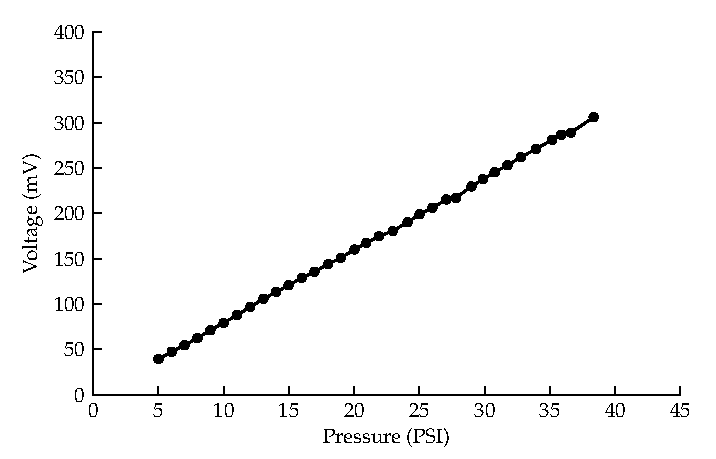
\includegraphics{content/pt1/01-PowerHarvesting/graphics/streamingCell_voltVsPress_52um_out}
    \caption{\label{fig:streamingCell_voltVsPress_52um_convienient}Line graph
        showing voltage output versus pressure for a 52$\,\mu m$ glass
        micro-channel.} \end{figure}


From the results obtained it is clear that there is a definite \nobreakdash-
linear \nobreakdash- relationship between the amount of pressure applied and
the voltage developed across each channel. Figure
\ref{fig:streamingCell_scatter_voltGradVsHeight} compares the gradient of
voltage developed per PSI of pressure for each of the channels. The graph shows
a trend toward larger voltage development as channel height is reduced to
around 50$\,\mu m$. Below 50$\,\mu m$ it is unclear what to expect from the
channel which will require further investigation. Spread in the data is
expected to be the result of epoxy (used to glue the slides together) seeping
into the cavity, thereby slightly altering each cavity's dimensions.

\begin{figure} \begin{centering}
        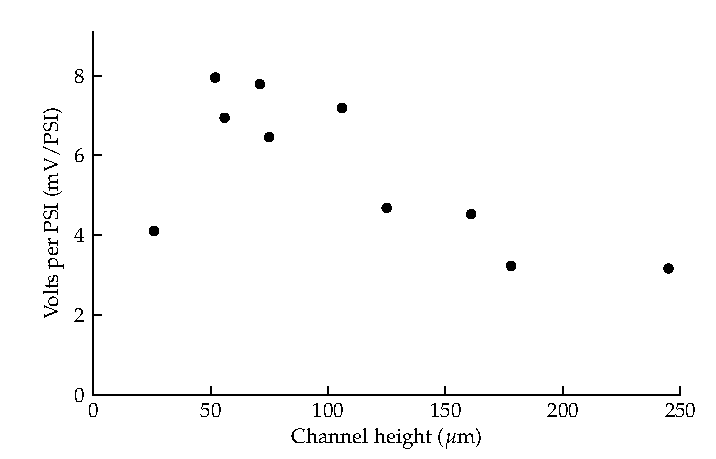
\includegraphics{content/pt1/01-PowerHarvesting/graphics/streamingCell_slopeVsChannelHeight}
        \par\end{centering}

\protect\caption{\label{fig:streamingCell_scatter_voltGradVsHeight}Scatter plot
    of voltage/pressure gradient versus channel height for each of the measured
    channels.}


\end{figure}



\subsection{Conclusion}

Power generation from streaming potential cells is possible, this is evident
from the voltages developed in this experiment. The streaming cell is capable
of producing output when operated using standard tap water at standard tap
pressures. As yet, the amount of current that can be drawn from such a channel
has not been ascertained, and therefore the amount of available power remains
unknown (although it is estimated to be in the very small). An initial estimate
of the ideal channel lies between 25-75$\,\mu m$ in height.


\section{Governing model}


\subsection{Charge separation analysis}

As mentioned at the beginning of this chapter, for a streaming potential cell
to operate there must be an electrical potential at the interface between solid
and liquid matter. In the experiment that Wayne Crump and myself replicated,
the solid/liquid interface was between glass and standard Hamilton tap water,
so where does this electrical potential come from?

Quoting Tandon et al. in \cite{Tandon2008}: Many microfluidic substrates behave
as weak acids in aqueous solutions. In glass substrates, surface silanol groups
can be deprotonated in aqueous solutions leaving a negative surface charge:

\begin{equation}
    SiOH\overset{^{K_{a}}}{\mathbf{\rightleftharpoons}}SiO^{-}+H^{+}
\end{equation}


It is this deprotonation that is responsible for generating the charge
difference at the glass/liquid surface of the microchannel and therefore
establishing an electrical double layer (EDL). Since the charge imbalance in
this case arises from the fact that the glass behaves as a weak acid, the
process itself is affected by the pH of the liquid, something we have no
control over when using tap water.

Once an ionic double layer within the channel has been established, ``the
streaming potential is engendered by the flow of the ions relative to the
stationary charged wall of the channel'' \cite{Mansouri2005}.  This flow is
accomplished in our case by applying a pressure gradient across the channel.
``The ratio of streaming potential to pressure gradient depends on the zeta
potential''\cite{Park2009}


\subsection{\label{sub:StreamingCell-Mathematics}Mathematics}

The first step toward optimisation is to define all the parameters that
describe the device. The streaming current, which is defined as the electrical
current that flows in the direction of water flow, is defined in
\cite{Olthuis2005} to be:

\begin{equation} I_{s}=\frac{A\,\varepsilon_{0\,}\varepsilon_{r}}{\eta\,
        l}\Delta P\,\zeta\label{eq:StreamingCell_StreamingCurrentFunc}
\end{equation} where: \begin{description} \item [{$\varepsilon_{0}$}] is the
        permittivity of free space \item [{$\varepsilon_{r}$}] is the relative
        permittivity of the liquid \item [{$\eta$}] is the viscosity of the
        liquid \item [{$l$}] is the length of the channel \item [{$\Delta P$}]
        is the pressure difference across the channel \item [{$\zeta$}] is the
        zeta-potential of the of the glass-liquid interface \item [{$A$}] is
        the cross-sectional area of the channel, or combined area of multiple
        channels \end{description} This equation indicates that the cell will
produce a current that is proportional to the amount of pressure across it and
that the output is affected by the geometry of the channel itself. To help
model the situation it is convenient to break Equation
\ref{eq:StreamingCell_StreamingCurrentFunc} formula down in the following
manner: \begin{eqnarray} I_{s} & = & \Delta P\,\left(\frac{A}{\eta\,
            l}\right)\,\left(\varepsilon_{0}\,\varepsilon_{r}\,\zeta\right)\nonumber
    \\ I_{s} & = & \frac{\Delta P}{\left(\frac{\eta\,
                l}{A}\right)}\,\left(\varepsilon_{0}\,\varepsilon_{r}\,\zeta\right)\nonumber
    \\ I_{s} & = & \frac{\Delta
        P}{R_{h}}\,\left(\varepsilon_{0}\,\varepsilon_{r}\,\zeta\right)\label{eq:StreamingCurrent_HydrostaticResistance}\\
    \frac{I_{s}}{\Delta P} & = &
    \frac{\varepsilon_{0}\,\varepsilon_{r}\,\zeta}{R_{h}}\nonumber \\ g_{m} & =
    & \frac{\varepsilon_{0}\,\varepsilon_{r}\,\zeta}{R_{h}}\nonumber
\end{eqnarray}


where $R_{h}$ is the hydrodynamic resistance caused by the channel, $g_{m}$
represents the transconductance between pressure applied and current produced
and $I_{s}$ is the streaming current. The hydrodynamic resistance ($R_{h}$)
will be affected by the geometry of the channel so $R_{h}$ is considered an
approximation of the hydrodynamic resistance.

Once the cell begins to separate charge a current in the reverse direction is
established called the conduction current ($I_{c}$).

Ohms law states:

\[ I=\frac{V}{R} \]


In this situation the resistance is determined by the conductivity of the water
($\sigma$), as well as the cross sectional area ($A$) and length ($l$) of the
channel.

\[ R=\frac{l}{\sigma\, A} \]


Therefore, the conduction current back through the channel is determined by:

\begin{equation} I_{c}=A\sigma\frac{V_{s}}{l} \end{equation}


Where $\sigma$ is the conductivity of the liquid and $V_{s}$ is the voltage
developed across the channel. This is also shown in

At equlibrium the streaming current ($I_{s}$) and the conduction current
($I_{c}$) are equal and opposite in direction.


\subsection{\label{sub:Electrical-model}Electrical model}

Figure \ref{fig:StreamingCell_Schematic-representation} depicts schematically
how a streaming cell would operate when connected to an external load.  This
model is based upon that found in \cite{Olthuis2005} by Olthuis et al. but has
been modified to show the pressure applied ($\Delta P$) as the voltage source,
instead of the zeta potential ($\zeta$). It is the pressure that responsible
for creating the streaming current; a zeta potential on its own simply isn't
enough. This has been shown through the results obtained in Appendix
\ref{sec:Appendix-Streaming-Potential-Cell}, where $V_{s}$ was directly
proportional to $\Delta P$; as $V_{s}$ is directly related to $I_{s}$ as per
Ohm's law.

\begin{figure} \begin{centering}
        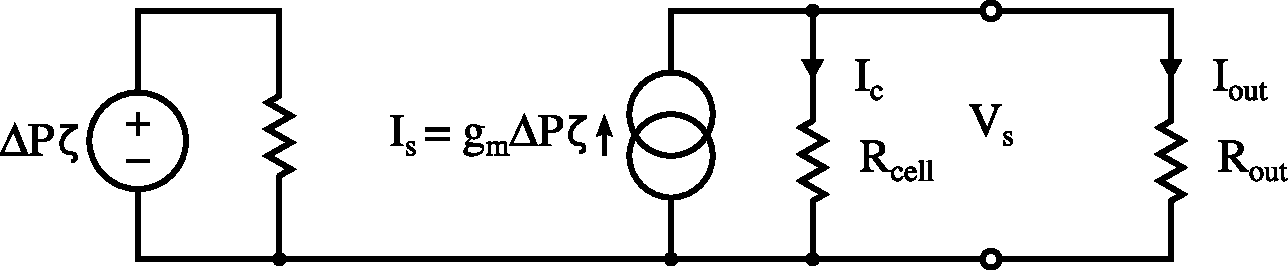
\includegraphics[scale=0.55]{content/pt1/01-PowerHarvesting/graphics/StreamingCell_EquivalentCircuit_output}
        \par\end{centering}

\protect\caption{\label{fig:StreamingCell_Schematic-representation}Schematic
    representation of a streaming cell with attached output resistance}
\end{figure}



\subsection{Output analysis}

The electrical model described in \ref{sub:Electrical-model} shows how the cell
would operate with a load placed across the cell. By combining this model with
the equations from \ref{sub:StreamingCell-Mathematics} it should be possible to
see the effect that altering various cell parameters has on the output.

\begin{eqnarray} P & = & V\times I\nonumber \\ V & = & I\times R\nonumber \\ P
    & = & I^{2}\times R\nonumber \\ P_{out} & = & I_{out}^{2}\times
    R_{out}\nonumber \\ I_{out} & = &
    I_{s}\times\frac{R_{cell}}{R_{cell}+R_{out}}\nonumber \\ P_{out} & = &
    \left[I_{s}\times\frac{R_{cell}}{R_{cell}+R_{out}}\right]^{2}\times
    R_{out}\label{eq:DeterminingOutputPower} \end{eqnarray}



\subsubsection{Finding an optimum value for $R_{out}$}

Using Ohm's Law it is possible to find an equation that give the output power
as a function of the electrical resistance of the cell ($R_{cell)}$) and the
output resistance ($R_{out}$) as shown in Equation
\ref{eq:DeterminingOutputPower}.  In order to optimise the output power it is
necessary to find the value of output resistance ($R_{out}$) that maximises the
output power.

Next I take Equation \ref{eq:DeterminingOutputPower} and treat the streaming
current ($I_{s}$) as a constant, differentiate with respect to $R_{out}$ and
find the condition that gives a maximum/minimum power output.

\begin{eqnarray*} \frac{\partial P_{out}}{\partial R_{out}} & = &
    \frac{R_{cell}^{2}}{(R_{cell}+R_{out})^{2}}-\frac{2\times
        R_{cell}^{2}\times R_{out}}{(R_{cell}+R_{out})^{3}}\\ 0 & = &
    \frac{R_{cell}^{2}}{(R_{cell}+R_{out})^{2}}-\frac{2\times
        R_{cell}^{2}\times R_{out}}{(R_{cell}+R_{out})^{3}}\\ \frac{2\times
        R_{cell}^{2}\times R_{out}}{(R_{cell}+R_{out})^{3}} & = &
    \frac{R_{cell}^{2}}{(R_{cell}+R_{out})^{2}}\\ \frac{2\times
        R_{cell}^{2}\times R_{out}}{R_{cell}+R_{out}} & = & R_{cell}^{2}\\
    2\times R_{cell}^{2}\times R_{out} & = &
    R_{cell}^{2}\times(R_{cell}+R_{out})\\ 2\times R_{out} & = &
    R_{cell}+R_{out}\\ R_{out} & = & R_{cell} \end{eqnarray*}


This shows that there is either maximum or minimum power transfer to $R_{out}$
when the value of $R_{out}$ matches that of $R_{cell}$, which is shown to be a
maximum as per Figure \ref{fig:Plot-of-PowerThereom}.  This result is
consistant with that of the Maximum Power Thereom, which I had trouble finding
a reference of for a current source and resistances in parallel. It shows that
in order to achieve the maximum possible output power, that the load should
have a resistance equal to that of the electrical resistance of the cell
itself. Additionally, it was found that the absolute magnitudes of both
$R_{out}$ and $R_{cell}$ have no effect on the output power, so long as they
are equal to one another.

\begin{figure}
    \begin{centering}
        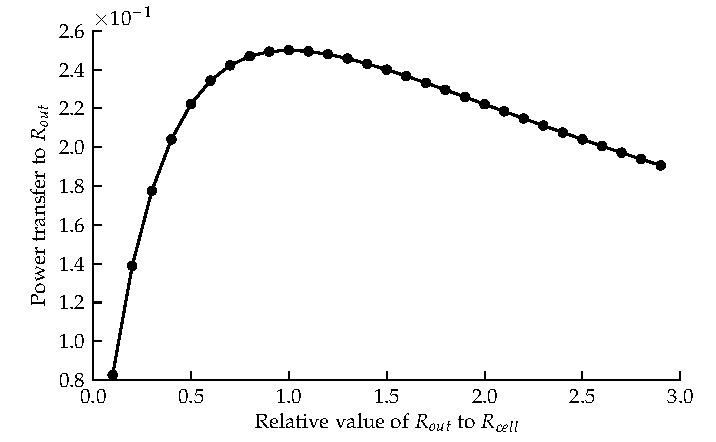
\includegraphics{content/pt1/01-PowerHarvesting/graphics/maximumPowerThereom}
    \end{centering}
    \caption{\label{fig:Plot-of-PowerThereom}Plot of Equation \ref{eq:DeterminingOutputPower} when $I_{s}=1A$ and $R_{cell}=1\Omega$}
\end{figure}


This can now be used to calculate the maximum available power as a function of
$I_{s}$ by substituting $R_{out}$ and $R_{cell}$ for $R$ , as
$R_{out}=R_{cell}=R$:

\begin{eqnarray} P_{out} & = &
    \left[I_{s}\times\frac{R_{cell}}{R_{cell}+R_{out}}\right]^{2}\times
    R_{out}\nonumber \\ P_{max} & = &
    \left[I_{s}\times\frac{1}{2}\right]^{2}\times R\nonumber \\ P_{max} & = &
    \frac{I_{s}^{2}R}{2}\label{eq:streamingCell_maxPower} \end{eqnarray}


And as $P=I^{2}R$ (via the power equation and Ohm's Law) this indicates that at
most we can hope to havest half of the total power, while the other half is
dissipated back through $R_{cell}$. Combining Equations
\ref{eq:streamingCell_maxPower} and
\ref{eq:StreamingCurrent_HydrostaticResistance} gives:

\begin{eqnarray*} P_{max} & = & \frac{\left(\frac{\Delta
                P}{R_{h}}\,\left(\varepsilon_{0}\,\varepsilon_{r}\,\zeta\right)\right)^{2}R}{2}\\
    P_{max} & = & \frac{\left(\frac{\Delta
                P\,\varepsilon\,\zeta}{R_{h}}\right)^{2}R}{2}\\ P_{max} & = &
    \frac{\Delta P^{2}\,\varepsilon^{2}\,\zeta^{2}R}{2R_{h}^{2}}
\end{eqnarray*}


where $\varepsilon=\varepsilon_{0}\,\varepsilon_{r}$ and $R=R_{cell}=R_{out}$ .
If we now substitute $R$ and $R_{h}$ for their respective functions we end up
with:

\begin{eqnarray} P_{max} & = & \frac{\Delta
        P^{2}\,\varepsilon^{2}\,\zeta^{2}R}{2R_{h}^{2}}\nonumber \\ P_{max} & =
    & \frac{\Delta P^{2}\,\varepsilon^{2}\,\zeta^{2}\,\left(\frac{l}{\sigma\,
                A}\right)}{2\left(\frac{\eta\, l}{A}\right)_{h}^{2}}\nonumber
    \\ P_{max} & = & \frac{\Delta P^{2}\,\varepsilon^{2}\,\zeta^{2}\,
        l}{\sigma\, A}\times\frac{1}{\frac{2\eta^{2}\, l^{2}}{A^{2}}}\nonumber
    \\ P_{max} & = & \frac{\Delta P^{2}\,\varepsilon^{2}\,\zeta^{2}\, l\,
        A^{2}}{\sigma\, A\,2\eta^{2}\, l^{2}}\nonumber \\ P_{max} & = &
    \frac{\Delta P^{2}\,\varepsilon^{2}\,\zeta^{2}\, A}{2\,\sigma\,\eta^{2}\,
        l}\nonumber \\ P_{max} & \propto & \frac{\Delta P^{2}\,\zeta^{2}\,
        A}{l}\nonumber \\ P_{max} & \propto & \frac{\Delta
        P^{2}\,\zeta^{2}}{R_{h}} \end{eqnarray}



\subsubsection{Optimisation of $R_{h}$ and $\Delta P$}

Knowing the optimum value of output resitance leaves only the streaming current
($I_{s}$) and it's constituants as optimisation parameters.  Equation
\ref{eq:StreamingCurrent_HydrostaticResistance} indicates that in order to
further optimise the cell, one must reduce hydrodynamic resistance ($R_{h}$)
and increase both the Zeta potential ($\xi$) and pressure difference ($\Delta
P$) placed across the cell.

We can model the water supply, harvester and a consumer as a basic electrical
circuit as shown in Figure \ref{fig:Schematic-model-of-harvester}.  In this
model $P_{supply}$ represents the total water pressure available, Flow
represents the flow rate of water, $R_{h}$ and $R_{consumer}$ are the
hydrodynamic resistances of the harvesting cell and a water consumer (e.g. a
house) respecively and $\Delta P$ is the pressure developed difference across
the harvester, where $R_{h}\propto\frac{l}{A}$.

\begin{figure} \begin{centering}
        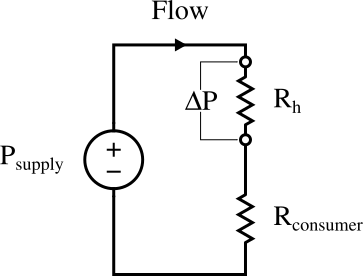
\includegraphics[scale=0.55]{content/pt1/01-PowerHarvesting/graphics/Harvester_equivalentCircuit_output}
        \par\end{centering}

\protect\caption{\label{fig:Schematic-model-of-harvester}Schematic model of the
    water supply, harvester and consumer}


\end{figure}


\begin{figure} \begin{centering}
        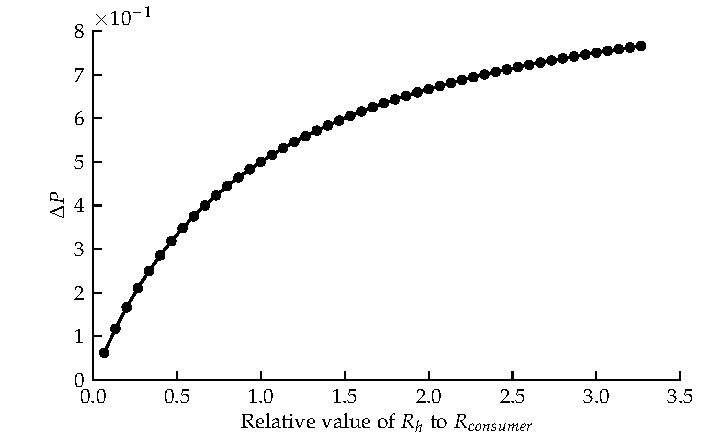
\includegraphics{content/pt1/01-PowerHarvesting/graphics/streamingCell_consumerModel_dP}
        \par\end{centering}

\protect\caption{\label{fig:Effect-of-varying-Rh-onP}Effect of varying $R_{h}$
    on $\Delta P$ for the harvester/consumer model shown in Figure
    \ref{fig:Schematic-model-of-harvester}.}


\end{figure}


\begin{figure} \begin{centering}
        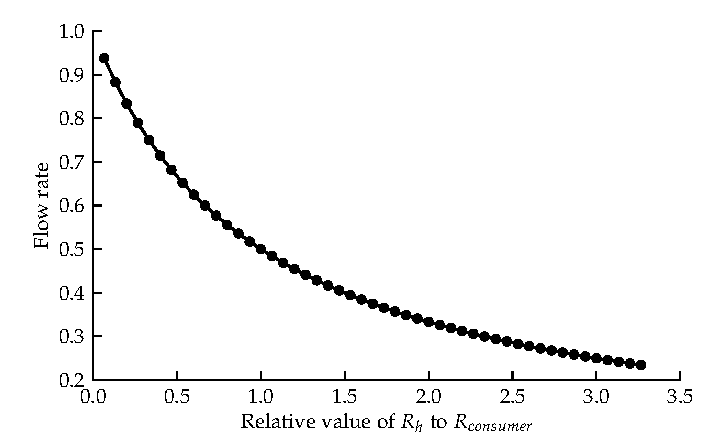
\includegraphics{content/pt1/01-PowerHarvesting/graphics/streamingCell_consumerModel_flow}
        \par\end{centering}

\protect\caption{\label{fig:Effect-of-varying-Rh-onFlow}Effect of varying
    $R_{h}$ on Flow for the harvester/consumer model shown in Figure
    \ref{fig:Schematic-model-of-harvester}.} \end{figure}


\begin{figure} \begin{centering}
        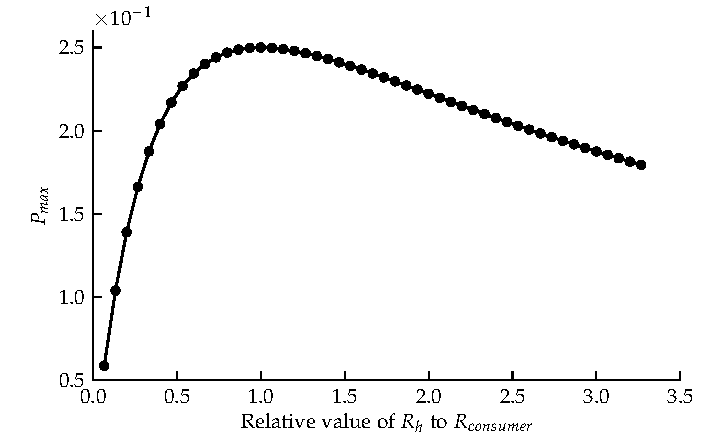
\includegraphics{content/pt1/01-PowerHarvesting/graphics/streamingCell_consumerModel_total}
        \par\end{centering}

\protect\caption{\label{fig:Effect-of-varying-Rh-onIs}Effect of varying $R_{h}$
    on \foreignlanguage{english}{$P_{max}$} for the harvester/consumer model
    shown in Figure \ref{fig:Schematic-model-of-harvester}.} \end{figure}
Figures \ref{fig:Effect-of-varying-Rh-onP},
\ref{fig:Effect-of-varying-Rh-onFlow} and \ref{fig:Effect-of-varying-Rh-onIs}
show how varying $R_{h}$ will affect $\Delta P$, the flow rate and the value of
$\frac{\Delta P}{R_{h}}$ respectively. Notice in Figure
\ref{fig:Effect-of-varying-Rh-onP} that increasing $R_{h}$ has the effect of
increasing $\Delta P$.  Optimisation wise, the benifit of increasing $I_{s}$ by
increasing $\Delta P$ is opposed by also increasing the value of $R_{h}$
(referring to Equation \ref{eq:StreamingCurrent_HydrostaticResistance}).

Figure \ref{fig:Effect-of-varying-Rh-onFlow} shows how the value of $R_{h}$
affects the flow rate through the system. Keeping the flow rate high is
important in order to ensure that the consumer does not notice a drop in water
pressure due to the addition of the harvester in their water system.

Finally, Figure \ref{fig:Effect-of-varying-Rh-onIs} shows the effect that
varying $R_{h}$ has on \foreignlanguage{english}{$P_{max}$} (according to
$P_{max}\propto\frac{\Delta P^{2}\,\zeta^{2}}{R_{h}}$ when $\zeta=1$). The
result is the same as that of Equation \ref{eq:DeterminingOutputPower}, showing
that this is again goverend by the maximum power transfer thereom. Practically,
a harvester that dropped half of the supply pressure would not be feasable in
most domestic situations, so a trade-off will have to be made that meets
plumbing standards.


\subsubsection{Optimisation of the Zeta potential}

Referring back to Equation \ref{eq:StreamingCell_StreamingCurrentFunc}, I have
determined how to increase the total output of the harvester by choosing
appropriate values for all of the parameters except $\varepsilon_{r}$ and
$\zeta$. As the harvester will be using domestic tap water the value of
$\varepsilon_{r}$ will be that of the relative permittivity of water, and is
therefore relatively fixed (being only affected by the temperature of the
water). This leaves $\zeta$ as the remaining parameter.

